\chapter{Adders}
\label{ch:adders}

%%\textit{ripple-carry adders, twos complement, subtraction, \dots}

\section{Addition by Numeral}
\label{sec:addition-by-numeral}

When people do paper-and-pencil arithmetic,
they do it using numerals.
For example, to add two numbers, a person
writes down the decimal numerals for the numbers,
one under the other with the digits lined up so that
the units digit of one number is directly under
the units digit of the other, and similarly for
the tens digits, hundreds digits, and so on.
Then, the units digits are added together,
and the low-order digit of that sum is written
in the units-digit column.

If the sum of the units digit is ten or more,
a "carry" is indicated in the tens-digit column.
The sum of the tens digits is computed and the
carry added to the sum if there was a carry.
As before, the low-order digit of the sum of the
tens digits (and carry) goes in the numeral for the sum,
but this time in tens-digit column.
A carry is marked, if necessary,
in the hundreds digit column.
This process moves across the digits of the summands until all the digits
are accounted for (Figure~\ref{fig:adding-decimal-numerals}).

\begin{figure}
\begin{lstlisting}
   11 1    carries
    ----
    9542   summand A
  +  638   summand B
    ----
   10180   sum A+B
\end{lstlisting}
\caption{Adding Decimal Numerals}
\label{fig:adding-decimal-numerals}
\end{figure}

To perform addition in this way, a person needs to know
the table for one-digit sums (0+0=0, 0+1=1, \dots 2+2=4 \dots 9+8=17, 9+9=18).
There are a hundred entries in the table ($10 \times 10$, one for each
possible pair of decimal digits).

Decimal numerals are not the only kind,
and addition can be carried out similarly, regardless of numeral base.
The table of one-digit sums is, of course, much smaller for binary numerals
than for decimal numerals.
It has only four entries ($0+0=0, 0+1=1, 1+0=0, 1+1=10_2$).
Except for the new, smaller table for one-digit sums,
the process is the same (Figure~\ref{fig:adding-binary-numerals}).

\begin{figure}
\begin{lstlisting}
   11 111 1    carries
    --------
    01011101   summand A
  + 11010101   summand B
    --------
   100110010   sum A+B
\end{lstlisting}
\caption{Adding Binary Numerals}
\label{fig:adding-binary-numerals}
\end{figure}

The small size of the one-digit-sum table simplifies the
both pencil-and-paper process and the difficulty of designing
digital circuits for performing addition on binary numerals, compared to what
it would be for decimal numerals.

\begin{ExerciseList}
\Exercise Describe by example the process of multiplying a pair of decimal numerals.

\Exercise Describe by example the process of multiplying a pair of binary numerals.
\end{ExerciseList}

\section{Adding One-Bit Binary Numerals}
\label{sec:adding-1-bit-numerals}

The addition table for one-bit, binary numerals
has only four entries, as shown in
Figure~\ref{fig:1-bit-add-table}.
In the figure, the sum is shown in all four cases as two separate bits,
a carry bit $c$ and a sum bit $s$.

\begin{figure}
\begin{center}
\begin{tabular}{|c|c|c|c}
 \hline
 $x+y$  & $c$ & $s$ \\
 \hline
 $0+0$  & $0$ & $0$ \\
 \hline
 $0+1$  & $0$ & $1$ \\
 \hline
 $1+0$  & $0$ & $1$ \\
 \hline
 $1+1$  & $1$ & $0$ \\
 \hline
\end{tabular}
\end{center}
\caption{One-Bit Addition Table}
\label{fig:1-bit-add-table}
\end{figure}

A close look at the table shows that
the carry bit matches the table of values of the
digital gate for logical-and (Figure \ref{fig-02-logic-gates}).
That is, the carry bit is 1 only if both inputs are 1s.
Otherwise, the carry bit is 0.
So, constructing a digital circuit to compute the carry bit
in the addition of two one-bit, binary numerals is simply
a matter of feeding the signals for the one-bit numerals
into a logical-and gate.

Another close look reveals that the sum bit
matches the table of values of the
digital gate for exclusive-or (Figure \ref{fig-02-logic-gates}).
That is, the sum bit is 0 if the two inputs are the same
and 1 if they are different.
So, constructing a digital circuit to compute the sum bit
amounts to feeding the signals for the one-bit numerals
into an exclusive-or gate.
Combining these ideas for carry-bit and sum-bit circuits
leads to a two-input, two-output circuit known as a
half-adder (Figure \ref{fig:half-adder}).

\begin{figure}
\begin{center}
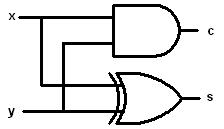
\includegraphics[scale=0.7]{Images/half-adder.png}
\todo{Improvised with PowerPoint. Redraw using Visio.}
\begin{tabular}{|c|c|c|c}
 \hline
 $x+y$  & $c$ & $s$ \\
 \hline
 $0+0$  & $0$ & $0$ \\
 \hline
 $0+1$  & $0$ & $1$ \\
 \hline
 $1+0$  & $0$ & $1$ \\
 \hline
 $1+1$  & $1$ & $0$ \\
 \hline
\end{tabular}
\end{center}
\caption{Half-Adder Circuit}
\label{fig:half-adder}
\end{figure}

Since we reason about digital circuits using the methods
of Boolean algebra, we need an algebraic representation
of the circuit-diagram for the half-adder circuit.
Remember, digital circuits are only one of four
equivalent representations of Boolean formulas that
we have studied: circuit diagrams, well-formed formulas
in the notation of mathematical logic (for example, $x \wedge y$),
Boolean formulas in engineering notation (justaposition for $\wedge$,
$+$ for $\vee$, and over-bar for $\neg$), and ACL2 notation.

The ACL2 form allows us to take advantage
of the mechanization of some aspects of the reasoning process.
So, we specify the half-adder circuit in ACL2 terms
(Figure \ref{fig:half-adder-acl2})
and refer to this specification as an
ACL2 model of the half-adder circuit.
It delivers the two output signals as a list of two elements,
the first element being the sum bit and the second, the carry bit.

\begin{figure}
\begin{lstlisting}
(defun and-gate (x y) (if (and (= x 1) (= y 1)) 1 0))
(defun xor-gate (x y) (if (= x y) 0 1))
(defun half-adder (x y) (list (xor-gate x y) (and-gate x y)))
\end{lstlisting}
\caption{ACL2 Model of Half-Adder Circuit}
\label{fig:half-adder-model}
\end{figure}

In the end, we would like to have a circuit
that adds binary numerals,
and we saw in an example (Figure \ref{fig:adding-binary-numerals})
that this would require us to deal with three input bits
for each bit in the numerals:
the corresponding bits in the two summands (ones-bit, twos-bit,
fours-bit, \dots) and the carry bit from the previous column.

The half-adder circuit is not up to this task,
since it has only two input signals.
However, we can put together a ``full-adder circuit''
by combining two half-adders with an or-gate,
as shown in the circuit of Figure \ref{fig:full-adder}.
Since the full-adder circuit has three inputs,
each of which is either 0 or 1,
there are exactly eight possible input configurations.
We could build a comprehensive verification of
the ACL2 model of the full-adder
circuit of Figure \ref{fig:full-adder} by writing
eight check-expect tests matching the full-adder table.

\begin{lstlisting}
(check-expect (full-adder 0 0 0) (list 0 0))
(check-expect (full-adder 0 0 1) (list 1 0))
  ...
(check-expect (full-adder 1 1 0) (list 0 1))
(check-expect (full-adder 1 1 1) (list 1 1))
\end{lstlisting}

Another approach is to observe
that the input combinations
match the list of binary numerals for the numbers 0 through 7,
padded with leading zeros to make them all have exactly three bits.
The function ``twos'' (page \pageref{twos-defun}) produces these numerals.

However, that approach is tedious, and it's easy to make a mistake.
Another approach is to observe that
the value delivered by (full-adder $c_{in}$ $x$ $y$)
is a binary numeral for the number $c_{in} + x + y$,
padded with a leading zero if necessary to make it have exactly two bits.
Since the function ``twos'' (page \pageref{twos-defun}) produces padded
numerals of that form, we expect that
(twos 2 (+ $c_{in}$ $x$ $y$)) = (full-adder (list $c_{in}$ $x$ $y$)).
In other words, making sure this equation holds
for each combination of values for $c_{in}$, $x$, and $y$
is the same as running the above check-expect tests.

\begin{figure}
\begin{center}
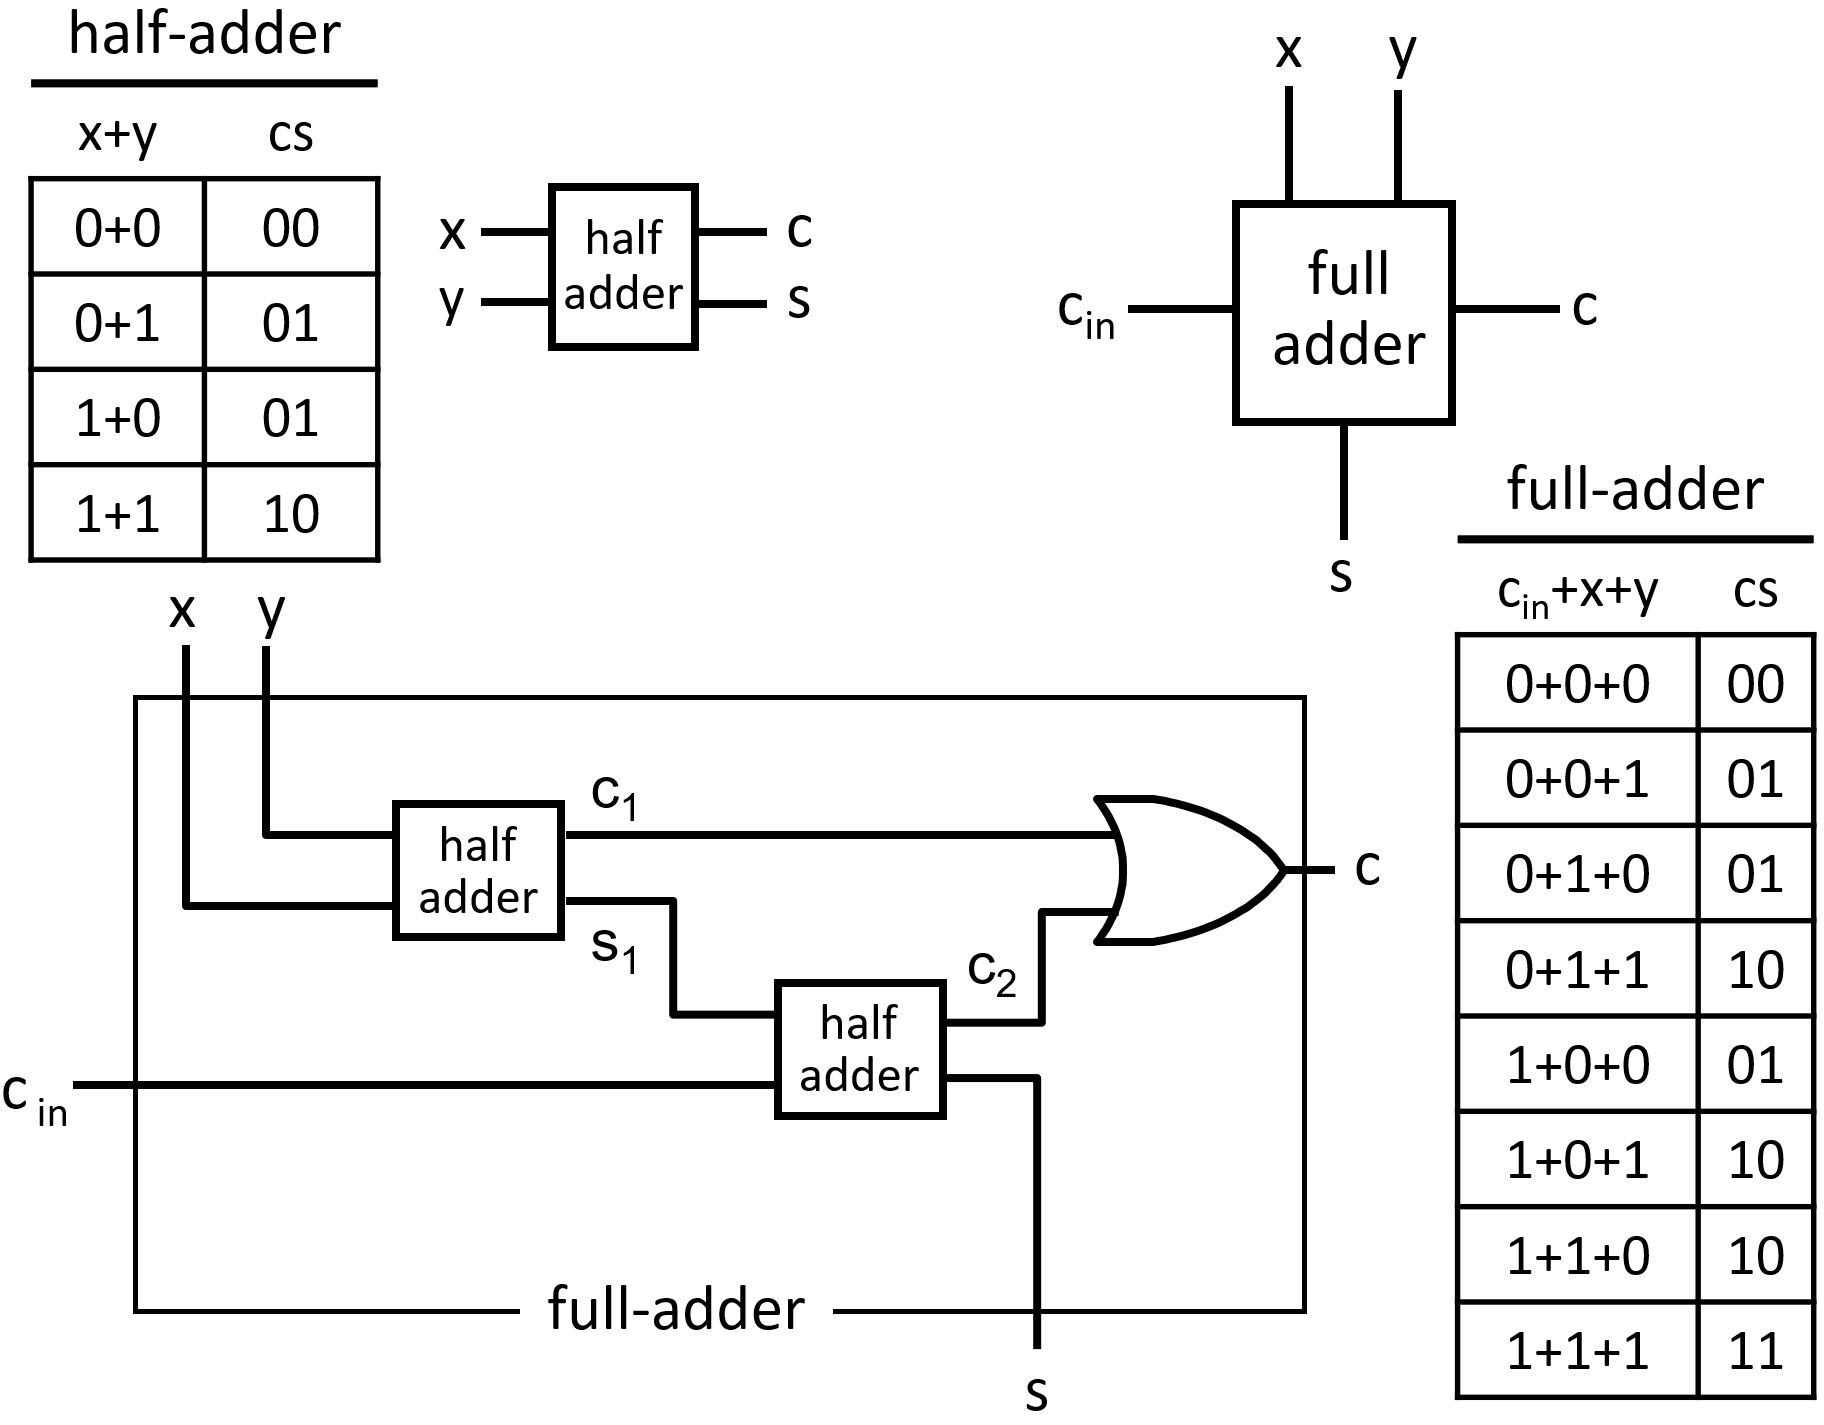
\includegraphics[scale=0.9]{Images/full-adder.png}
\todo{Improvised with PowerPoint. Redraw using Visio.}
\begin{lstlisting}
(defun and-gate (x y) (if (and (= x 1) (= y 1)) 1 0))
(defun or-gate (x y) (if (or (= x 1) (= y 1)) 1 0))
(defun xor-gate (x y) (if (= x y) 0 1))
(defun half-adder (x y) (list (xor-gate x y) (and-gate x y)))
(defun full-adder (c-in x y)
  (let* ((h1 (half-adder x y))
         (s1 (first h1))
         (c1 (second h1))
         (h2 (half-adder s1 c-in))
         (s  (first h2))
         (c2 (second h2))
         (c  (or-gate c1 c2)))
    (list s c)))
\end{lstlisting}
\end{center}
\caption{Full-Adder Circuit and ACL2 Model}
\label{fig:full-adder}
\end{figure}

Furthermore, the set of combinations of values for $c_{in}$, $x$, and $y$
is the same as the set of numerals for the numbers 0 through 7
padded with leading zeros to make them all have exactly three bits.
That is, the bit-combinations in the numerals
(twos 3 0), (twos 3 1), (twos 3 2), \dots (twos 3 7) comprise
the full set of combination of values for $c_{in}$, $x$, and $y$.
Therefore, each of the equations we want to check
has the form (chk-combo $n$), for some $n$ between 0 and 7,
where the function ``chk-combo'' is defined in
Figure \ref{fig:full-adder-model-check}.
That is, the ACL2 model of full-adder in Figure \ref{fig:full-adder}
is correct if all of the formulas following formulas are true:
(chk-combo 0), (chk-combo 1), (chk-combo 2), \dots (chk-combo 7).
We conclude that the constant\footnote{Constants in ACL2
are defined like functions, but with the keyword ``defconst'' instead
of ``defun''. Names of constants are required to start and end with asterisks,
and constants do not have parameters.}
``*chk-full-adder*'' defined in
Figure \ref{fig:full-adder-model-check} is true if the full-adder model
is correct and false if it isn't.

\begin{figure}
\begin{center}
\begin{lstlisting}
(defun chk-combo (n)
  (let* ((bit-combo (twos 3 n))
         (c-in (first bit-combo))
         (x    (second bit-combo))
         (y    (third bit-combo)))
    (equal (twos 2 (+ c-in x y))
           (full-adder c-in x y))))
(deconst *chk-full-adder* ; true iff full-adder model is correct
  (and (chk-combo 0) (chk-combo 1) (chk-combo 2) (chk-combo 3)
       (chk-combo 4) (chk-combo 5) (chk-combo 6) (chk-combo 7)))
\end{lstlisting}
\end{center}
\caption{Mechanized Verification of Full-Adder Model}
\label{fig:full-adder-model-check}
\end{figure}

We now have a fully mechanized verification
of the ACL2 model of the full-adder circuit.
That makes it safe to use this model as a component
in the design of a circuit to carry out addition on binary numerals
with more than one bit.

\section{Adding Two-Bit Binary Numerals}
\label{sec:adding-2-bit-numerals}

Adding binary numerals with two bits is simply a matter
of connecting two full-adder circuits in a manner that
directs the carry from adding the low-order bits
to the carry-input of the second full-adder circuit.
Since there is never a carry into the low-order position,
we just supply zero as the carry-in for the full-adder circuit
that deals with the low-order bit.

\begin{figure}
\begin{center}
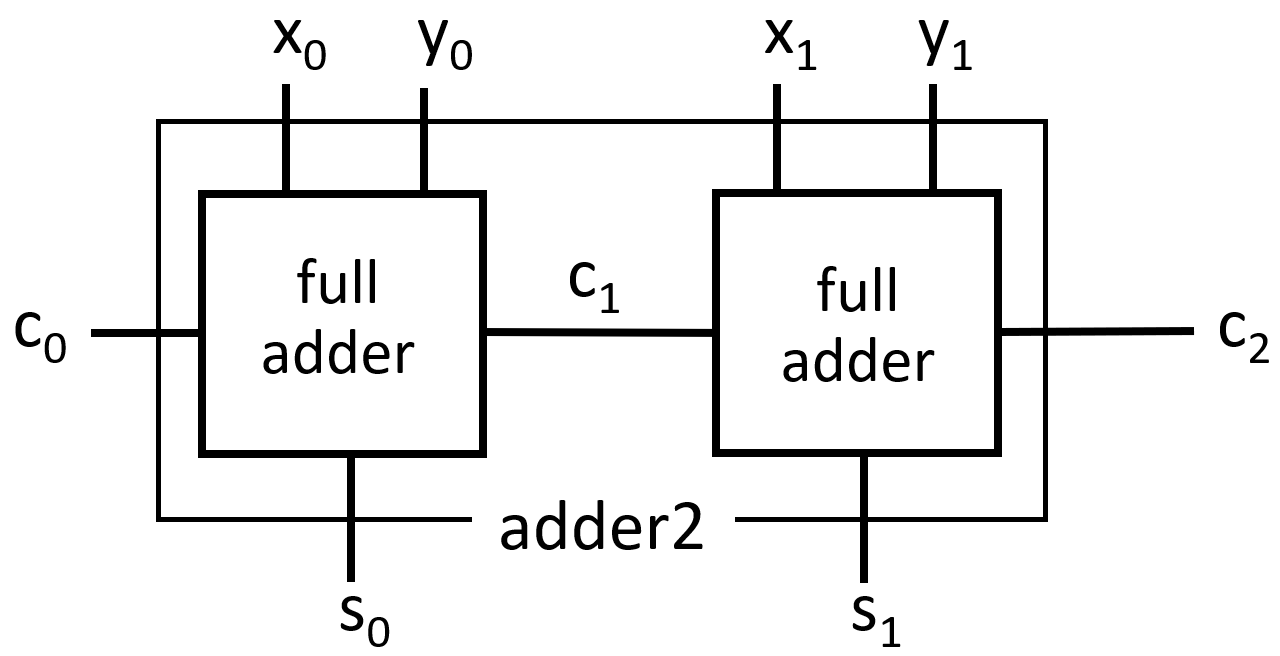
\includegraphics[scale=0.9]{Images/adder2.png}
\todo{Improvised with PowerPoint. Redraw using Visio.}
\begin{lstlisting}
(defun adder2 (c0 x y)
  (let* ((x0 (first x)) (x1 (second x))
         (y0 (first y)) (y1 (second y))
         (a0 (full-adder c0 x0 y0))
         (s0 (first a0)) (c1 (second a0))
         (a1 (full-adder c1 x1 y1))
         (s1 (first a1)) (c2 (second a1)))
    (list (list s0 s1) c2)))
\end{lstlisting}
\end{center}
\caption{Two-Bit Adder and ACL2 Model}
\label{fig:adder2}
\end{figure}

This two-bit addition circuit takes two, two-bit binary numerals
($x_0$ $x_1$) and ($y_0$ $y_1$) as inputs, and
delivers a two-bit numeral along with a carry-bit,
as shown in Figure \ref{fig:adder2} (\pageref{fig:adder2}).
We refer to the two-bit numeral without the carry bit
as the ``sum bits'' of the output from the two-bit adder.
There is also a carry bit.
Ignoring the carry bit amounts to doing
modular arithmetic, mod 4 ($2^2$), as is
confirmed by theorem \{\emph{pfx-mod}\} (page \pageref{pfx-mod}).

A mechanized verification of the correctness of the model
could be constructed in a manner similar to the one for one-bit addition
(Figure \ref{fig:full-adder-model-check},page \pageref{fig:full-adder-model-check}).
However, it would have 32 cases to check
because there are five bits of input in all
(a carry-in and two bits in each numeral, $2^5$ combinations in all).
That makes it tedious to construct, and it's easy to make a mistake.
A better way is to think of a formula in logic that expresses
the properties we expect the model to have.

One approach is to observe
the the numbers represented by the input
numerals, along with the input carry, must
add to the number represented by the output numeral (that is the sum bits),
with the output carry bit appended to the high-order bit position at the end.
Of course, the theorem will be stated as an implication, so that
we can constrain the inputs to be bits (zeros and ones),
and not some other kind of data.

To make it easy to state the constraints,
we define a Boolean function that delivers the value true
if its input is a bit and false otherwise.
The, stating the hypothesis of the implication
is just a matter of forming the logical-and
of tests that require the inputs to be bits.
The conclusion is the equation between the
sum of the numeric interpretation of the input numerals
(along with the input carry)
and the numeric interpretation of the output numeral
(with the output carry at the end).
Fortunately, we already have a trusted function
``num'' (page \pageref{num-defun})
that interprets binary numerals as numbers,
so we can use that function in the statement of
theorem \{\emph{adder-ok}\} specifying
the correctness of our model of the two-bit adder circuit.

\label{bitp-defun}
\begin{lstlisting}
(defun bitp (x)
  (or (= x 0) (= x 1)))

(defthm adder2-ok
  (implies (and (bitp c0) (bitp x0) (bitp x1)
                          (bitp y0) (bitp y1))
           (let* ((a (adder2 c0 (list x0 x1) (list y0 y1)))
                  (s (first a)) (c (second a)))
             (= (num (append s (list c)))
                (+ c0 (num (list x0 x1)) (num (list y0 y1)))))))
\end{lstlisting}
\label{adder2-ok}

\begin{ExerciseList}
\Exercise Define a doublecheck property that tests
for correctness of the two-bit adder model
(Figure \ref{fig:adder2}, page \pageref{fig:adder2}).
Run the test using Dracula.
Note: The data generator (random-between 0 1) delivers
a 0 or a 1 at random.

\Exercise By default, Dracula does fifty repeats
when it runs a doublecheck test.
How many tests with random data do you think would be needed to be reasonably
confident all 32 different cases for the two-bit adder have been tested?
\end{ExerciseList}

\section{Adding w-Bit Binary Numerals}
\label{sec:adding-w-bit-numerals}

By now, you can predict what a circuit for adding three-bit
binary numerals would look like.
Just put another full adder in the circuit, and feed the
carry from adding the two low-order bits into the carry-in
of the new full adder in the circuit, along with
the high-order bits in the two numerals.

Producing the circuit diagram for any number of bits
is just a matter of wiring the appropriate number of
full adders together in the appropriate way.
Figure \ref{fig:adder} (page \pageref{fig:adder}) presents a schematic for doing this.
The circuit is known as a ``ripple-carry adder'' because
of the way the carry-bit propagates across the line
of one-bit circuits.

\begin{figure}
\begin{center}
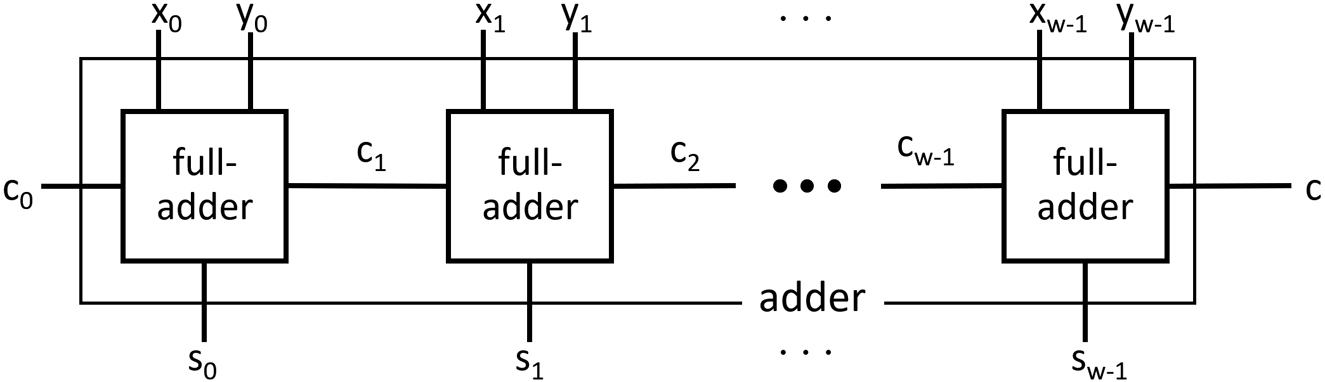
\includegraphics[scale=0.9]{Images/adder.png}
\todo{Improvised with PowerPoint. Redraw using Visio.}
\begin{lstlisting}
(defun adder (c0 x y)
  (if (consp x)
      (let* ((x0 (first x)) (y0 (first y))
             (a0 (full-adder c0 x0 y0))
             (s0 (first a0)) (c1 (second a0))
             (a  (adder c1 (rest x) (rest y)))
             (ss (first a)) (c (second a)))
        (list (cons s0 ss) c))
      (list nil c0)))
\end{lstlisting}
\end{center}
\caption{Ripple-Carry Adder and ACL2 Model}
\label{fig:adder}
\end{figure}

The ACL2 model in Figure \ref{fig:adder} ((page \pageref{fig:adder})) relies
on inductive definition. It feeds the carry-in and
the low-order bits from the two numerals into a full adder.
(The low-order bit in a numeral is the ``ones bit,''
which is the first element of the list that we use to
represent the numeral.)
The sum bit from that full adder
is the low-order bit of the numeral representing the sum of
the numbers that the input numerals represent.
The remaining bits in that sum are those delivered by
the adder operating on the other bits in the input numerals
(that is, all the bits in the input numerals except the low-order bits).

Because the model defines a function in ACL2,
you can run the function to see that it works in specific cases.
To add two binary numerals, supply lists of 0s and 1s
representing those numerals in an invocation
of the function ``adder'', and specify zero as the input carry-bit.
The output will be the numeral for the sum, mod $2^w$,
of the numbers that two input
numerals represent(where $w$ is the number of bits in the two numerals).
The output will also include a carry bit,
which will be zero if the sum of the two numbers is less than $2^w$.
It will be a one-bit if sum is $2^w$ or greater.

\begin{aside}
What if the input numerals have a different number of bits?
Suppose one of them has eight bits, and the other has ten.
The model is not designed to deal with that case.
We could change the design to accommodate input numerals
of differing lengths, but since we are modeling a circuit
in which the input numerals must both be of a specific length,
the model does not need to account for that possibility.
The issue of numerals of different lengths
is irrelevant in the context of the circuit.
\caption{Adder Circuit and Numerals of Different Lengths}
\label{adder-circuit-and-numerals-of-different-lengths}
\end{aside}

\begin{ExerciseList}
\Exercise Define in ACL2 a function ``add-bin''
that adds any two binary numerals,
even if the numerals contain a different number of bits.
That is, the value (add-bin $c$ $x$ $y$) should be a binary numeral
for the number (+ c (num $x$) (num $y$)),
as long as $x$ and $y$ are binary numerals and $c$ is 0 or 1,
regardless of (len $x$) or (len $y$).
Design and run some sanity checks (check-expect) on your function.

\Exercise Define in ACL2 a theorem that expresses the correctness
of the function ``add-bin'' from the previous exercise.
\end{ExerciseList}

\section{Adding Numerals for Negative Numbers}
\label{sec:adding-negative-numerals}

The ripple-carry adder circuit
(Figure \ref{fig:adder}, page \pageref{fig:adder})
provides a way to do addition entirely through numerals.
The inputs are numerals, and the output is a numeral.
Figure \ref{fig:adder-schematic} (page \pageref{fig:adder-schematic})
depicts the idea graphically,
throwing away the internal details
and ignoring the input carry bit and the output carry bit.

If the input carry is zero and
the input numerals are interpreted
as 2s-complement numerals for numbers in the set
$I(w) = \{-2^{w-1}, \dots -1, 0, 1, 2, \dots 2^{w-1}-1\}$,
then the output numeral (ignoring the carry) is the 2s-complement numeral
for the sum of the input numerals.
The theorem stated in
Figure \ref{fig:adder-schematic} (page \pageref{fig:adder-schematic})
formalizes this fact.

It is similar to the correctness theorem for the
model of the two-bit adder (page \pageref{adder2-ok}),
but the hypothesis of the implication must constrain
inputs to be binary numerals (that is, lists of bits).
An object is a list of bits if it is either
constructed by the cons operation in which the
first operand is a bit and the second operand
is a list of bits or if it is the empty list.
We define a Boolean function ``bit-listp'' to
encapsulate the idea of a list of bits.

\begin{figure}
\begin{center}
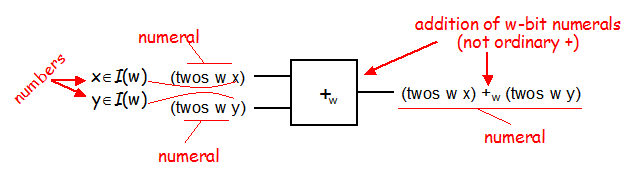
\includegraphics[scale=0.8]{Images/adder-schematic.png}
\todo{Improvised with PowerPoint. Redraw using Visio.}
\begin{lstlisting}
(defun bit-listp (xs)
  (if (consp xs)
      (and (bitp (first xs)) (bit-listp (rest xs)))
      (equal xs nil)))
(defthm adder-ok
  (implies (and (bitp c0) (bit-listp x) (bit-listp y)
                (= (len x) (len y)))
           (let* ((a (adder c0 x y))
                  (s (first a))
                  (c (second a)))
             (= (num (append s (list c)))
                (+ c0 (num x) (num y))))))
\end{lstlisting}
\end{center}
\caption{Adding 2s-Complement Numerals}
\label{fig:adder-schematic}
\end{figure}

Theorem \{\emph{adder-ok}\} (page \pageref{fig:adder-schematic})
states the correctness property that
we expect the adder circuit to satisfy.
We now turn our attention to proving that theorem.
Our proof will, of course, be about the model of the adder circuit
(Figure \ref{fig:adder}, page \pageref{fig:adder})
not the circuit itself.

\begin{aside}
We assume that our ACL2 models
accurately encode the circuits they represent.
In a full formalization, we would
need a way to convert models into instructions
for fabricating the circuits.
We expect that you could, given a basket of
logic gates, wires, and enough time,
use the diagram of the adder circuit to
build one for any specified word size,
and we think you can convince yourself that the model
matches the diagram.

Formalizing the construction of instructions a machine could
follow to fabricate a circuit, given an ACL2 model,
can be done using the methods
we have employed to formalize other operations.
But, in this treatment of the subject
we have left that step to the imagination.
\caption{Models and Circuit Fabrication}
\label{circuit-vs-model}
\end{aside}

\textit{proof goes here ...}

\begin{ExerciseList}
\Exercise Diagram a circuit that employs
the 2s-complement negation trick (Figure \ref{fig:2s-comp-negation},
page \pageref{fig:2s-comp-negation}) to deliver the
numeral for the negation of a number in the range
$\{-2^{w-1}+1, \dots -1, 0, 1, 2, \dots 2^{w-1}-1\}$
(that is, a number in the set $I(w)$ other than the
most negative number in that set).
You may assume that you have an adder circuit for
word-size $w$. Use the gate-like symbol
in Figure \ref{fig:adder-schematic} (page \pageref{fig:adder-schematic})
to depict that circuit in your diagram.

\Exercise Diagram a circuit that subtracts 2s-complement numerals.
You may assume that you have an adder circuit of word-size $w$
and a negation circuit (as in the preceding exercise).
Use the gate-like symbol
in Figure \ref{fig:adder-schematic} (page \pageref{fig:adder-schematic})
to depict that circuit in your diagram.
Make up a similar symbol to use for the negation circuit.

\Exercise Define an ACL2 model of a 2s-complement subtraction circuit.

\Exercise State a theorem that specifies the correctness of
a subtraction circuit for 2s-complement numerals.

\Exercise Design a comparison circuit that takes a pair of
2s-complement numerals as inputs and delivers the number 1
if the first number is smaller than the second
and the number 0 otherwise.
You may assume that you have an subtraction circuit of word-size $w$
as described in an earlier exercise. Make up a symbol to depict
that circuit in your diagram.
\emph{Hint}: Apply theorems \{\emph{minus-sign}\} and \{\emph{plus-sign}\}
(page \pageref{minus-sign}).

\Exercise Define an ACL2 model of a comparison circuit for 2s-complement numerals.

\Exercise State a theorem that specifies the correctness of
a comparison circuit for 2s-complement numerals.

\end{ExerciseList}

%%% Local Variables:
%%% mode: latex
%%% TeX-master: "book"
%%% End:
